\documentclass{article}

\usepackage{geometry}
\usepackage[T1]{fontenc}
\usepackage[utf8]{inputenc}
\usepackage{amssymb}
\usepackage{amsmath}
\usepackage{german}
\usepackage{pgf}

\usepackage{tikz}
\usetikzlibrary{arrows, automata}
\usetikzlibrary{positioning}

\usepackage{listings}
\usepackage{color}

\newcommand{\kreis}[1]{\unitlength1ex\begin{picture}(2.5,2.5)%
	\put(0.75,0.75){\circle{2.5}}\put(0.75,0.75){\makebox(0,0){#1}}\end{picture}}

\tikzset{
	state/.style={
			rectangle, rounded corners,
			draw=black,  thick, minimum height=2em, inner sep=2pt, text centered},
		}

\begin{document}
	\section{Rechenoperationen}
	\begin{enumerate}
		\item Baum besteht aus Knoten (Kreise) und Kanten (Pfeile)
		\item Kanten verbinden Knoten mit ihren Kind-Knoten
		\item jeder Knoten (außer der Wurzel) hat \underline{genau ein} Elternteil
		\item Knoten ohne Kinder heißen "'Blätter"' (leaf-nodes)
		\item Teilbaum
		\begin{enumerate}
			\item wähle beliebigen Knoten
			\item entferne temporär dessen Eltern-Kante
			\begin{enumerate}
				\item der Knoten wird temorär zu einer Wurzel
				\item dieser Knoten mit allen seinen Nachkommen bildet wieder seinen Baum - "' Teilbaum des Originalbaums"'
			\end{enumerate}
			\item Tiefe: Abstand des Knotens zur Wurzel
			\item 
		\end{enumerate}
	\end{enumerate}
	
	Infix-Notation: \\
	 $1+2+3*4/(1+5)-2$ \\ \\
	 Präfix-Notation: \\
	 $sub(add(add(1,2), div(mul(3,4), add(1,5))),2)$ \\ \\
	 
	 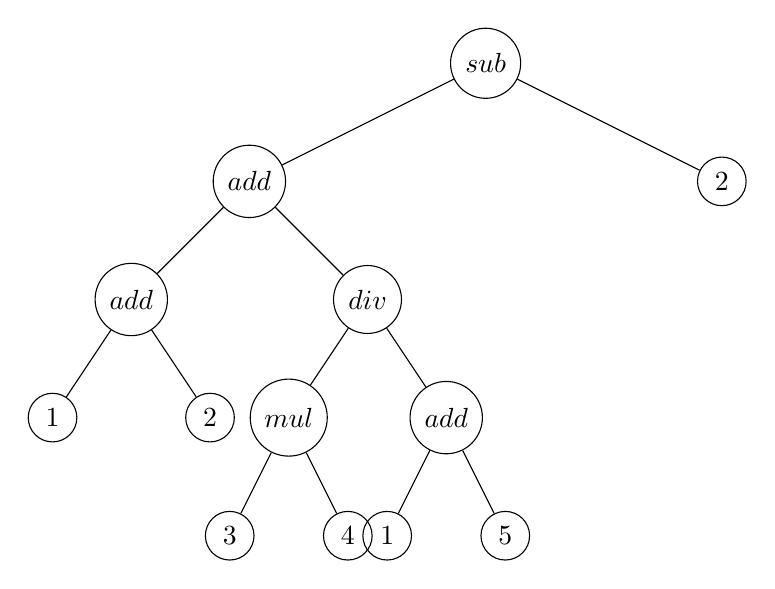
\begin{tikzpicture}[level/.style={sibling distance=60mm/#1}]
	 	
	 	\node [circle, draw] (z)  {$sub$}
	 	child {node [circle, draw] {$add$}
	 		child {node [circle, draw] {$add$}
	 			child{node [circle, draw] {$1$}}
	 			child{node [circle, draw] {$2$}}
	 		}
	 		child {node [circle, draw] {$div$}
	 			child{node [circle, draw] {$mul$}
	 				child {node [circle, draw] {$3$}}
	 				child {node [circle, draw] {$4$}}
	 			}
	 			child{node [circle, draw] {$add$}
	 				child {node [circle, draw] {$1$}}
	 				child {node [circle, draw] {$5$}}
	 			}
	 		}}
	 		child {node [circle, draw] {$2$}
	 		};
	 	\end{tikzpicture}
	 		
	\paragraph{Präfix Notation aus dem Baum rekonstruieren}
	 		
	 \begin{enumerate}
	 	\item Wenn die Wurzel ein Blatt ist, dann "'Drucke die Zahl"'
	 	\item sonst (Operator):
	 	\begin{enumerate}
	 		\item Drucke Funktionsnamen
	 		\item Drucke "'("'
	 		\item wiederhole ab $1)$ für das linke Kind
	 		\item Drucke "',"'
	 		\item wiederhole den Algorithmus ab $1)$ für das rechte Kind
	 		\item Drucke "')"'
	 	\end{enumerate}
	 \end{enumerate}
	
		Beachte Reihenfolge: Wurzel - Links - Rechts (Pre-Order Traversal)
		Ergebnis: \\
		$sub(add(add(1,2), div(mul(3,4), add(1,5))),2)$
		
		\paragraph{Definition: Rekursion}
		Rekursion meint Algorithmus für Teilproblem von vorn
		
		\paragraph{Infix Notation}
		
		\begin{enumerate}
			\item wie bei Präfix
			\item sonst
			\begin{enumerate}
				\item entfällt
				\item wie bei Präfix
				\item wie bei Präfix
				\item Drucke Operatorsymbol
				\item wie bei Präfix 
				\item wie bei Präfix
				\item wie bei Präfix
			\end{enumerate}
		\end{enumerate}
		Beachte Reihenfolge: Links - Wurzel - Rechts (In-Order Traversal) \newline
		
		Ergebnis: \\
		$(((1 + 2) + ((3 * 4)/(1 + 5))) + 2)$
		
		\paragraph{Berechne den Wert mit Substitutionsmethode}
		\begin{enumerate}
			\item Wenn Wurzel ein Blatt hat, gib die Zahl zurück
			\item sonst
			\begin{enumerate}
				\item entfällt
				\item entfällt
				\item wiederhole ab $1)$ für linken Teilbaum und speichere Ergebnis als "'left-result"'
				\item entfällt
				\item wiederhole ab $1)$ für rechten Teilbaum, speichere Ergebnis als "'right-result"'
				\item berechne $fkt_name(left-result, right-result)$ und gib Ergebnis zurück
			\end{enumerate}
		\end{enumerate}
		Beachte Reihenfolge: Links - Rechts - Wurzel (Post-Order Traversal)
		
		\begin{align*}
		&  	sub(add(add(1,2), div(mul(3,4), add(1,5))),2) \\
		= & \, sub(add(add(1,2), div(12, 6)),2) \\
		= & \, sub(add(3,2)2) \\
		= & \, sub(5,2) \\
		= & \, 3
		\end{align*}
		
		\section{Maschinensprache}
		\begin{itemize}
			\item optimiert für die Hardware (viele verschiedene)
			\item Gegensatz: höhere Programmiersprache ($C++$) ist optimiert für Programmierer
			\item Compiler oder Interpreter übersetzen Hoch- in Maschinensprache 
		\end{itemize}
		
		\paragraph{Vorgang des Übersetzens}
		\begin{enumerate}
			\item Eingaben (und Zwischenergebnisse) werden in Speicherzellen abgelegt $ \Rightarrow$ jeder Knoten im Baum bekommt eine Speicherzelle (Maschinensprache: durchnumeriert ; Hochsprache: sprechende Namen)
			\item Speicherzellen für die Eingaben $\underline{initialisieren}$ ; Notation: SpZ $\leftarrow$ Wert
			\item Rechenoperationen in der Reihenfolge des Substitutionsmodells ausführen und in der jeweiligen Speicherzelle speichern ; Notation: SpZ\_Ergebnis $\leftarrow$ fkt\_name SpZ\_Arg1 SpZ\_Arg2
			\item alles in Zahlencode umwandeln
			\begin{itemize}
				\item Funktionsname $\Rightarrow$ Opcodes
				\item Speicherzellen: nur die Nummer
				\item Werte sind schon Zahlen
				\item Notation: Opcode \quad Ziel SpZ \quad SpZ\_Arg1 \quad SpZ\_Arg2 oder Opcode \quad Ziel SpZ \quad Initialwert
			\end{itemize}
		\end{enumerate}
	
	\section{funktionale Programmierung}
	(alles durch Funktionsaufrufe ausführen)
	
	\begin{enumerate}
		\item bei Maschinensprache wurden Zwischenergebnisse in Speicherzellen abgelegt
		\item das ist auch in der funktionalen Programm. eine gute Idee
		\begin{enumerate}
			\item Speicherzellen werden durch Namen (vom Programmierer vergeben) unterschieden
			\item Beispiel: Lösen einer quadratischen Gleichung: $ax^2+bx+c =0$, finde $x_{1/2}$
					$\Rightarrow x^2-px+q =0 \quad mit \quad p = -\frac{b}{2a}, q = \frac{c}{a}$
					$\Rightarrow x_1 = -\frac{b}{2a} + \sqrt{(-\frac{b}{2a}^2 - \frac{c}{a})} \\ \Leftarrow allgemein: x_{1/2} = p \pm \sqrt{p^2-q}$
			\item Präfix: \\ $x_1 \leftarrow add(div(div(b,a),-2), sqrt(sub(mul(div(div(b,a),-2), div(div(b,a), -2)), div(c,a))))$ \\
					mit Zwischenergebnissen und Infix-Notation: $p \leftarrow b/c/-2 \quad $oder$ \quad p \leftarrow -0,5*b/a \quad q \leftarrow c/a$ \\ $discriminant \leftarrow sqrt(p*P-q)$ \\
					$x_{1/2} \leftarrow p \pm discriminant$
		\end{enumerate}
		\item zwei Vorteile:
		\begin{enumerate}
			\item lesbar
			\item redundante Berechnung verschieden \\ Beachte: In der funktionalen Programmierung können die Speicherzellen nach der Initialisierung \underline{nicht} mehr verändert werden
			\item Speicherzellen mit Namen sind nützlich, um Argumente an Funktionen zu übergeben $\Rightarrow$ Definition eigener Funktionen \\
			Bsp: 
			\framebox{function sq(x) \\
												\{
												return x*x
												\} }
		\end{enumerate}
	\end{enumerate}
	
	\section{funktionale Programmierung in C++}
	
	\begin{enumerate}
		\item in C++ hat jede Speicherzelle einen \underline{Typ} (legt Größe und Bedeutung der Speicherzelle fest) \\
		wichtigste Typen: \grqq int\grqq  für ganze Zahlen, \grqq double\grqq  für reelle Zahlen, \grqq std::string\grqq  für Text \\ zugehörige Literale (Konstanten): 12, -3 (int) \quad -1.02 , 1.2e-4 (double) \quad \grqq text text \grqq (string)
		\item Die Initialisierung wird geschrieben als
		\begin{lstlisting}[tabsize =2]
			type_name spz_name = initialwert
		\end{lstlisting}
		Bsp:
		\begin{lstlisting}[tabsize = 2]
			double a = 10
			std::cout << "x_1" << x_1 << "\n" ;
		\end{lstlisting} 
		\item eigene Funktion in $C++$: 

			\begin{lstlisting}[tabsize = 2]
			type_ergebnis funktionsname (typ_arg1 name_arg1, typ_arg2 name_arg2)
			{
				<code>
				return ergebnis;
			}
			\end{lstlisting}
			
		\item zwei Funktionen mit gleichem Namen, aber unterschiedlichen Typen dürfen in C++ gleichzeitig definiert sein (\grqq overloading\grqq) \\ $\Rightarrow$ C++ wählt \underline{automatisch} die richtige Variante anhand des Argumenttypes (\grqq overload resolution\grqq)
		
		\item jedes $C++$ -Programm muss \underline{genau eine} Funktion names \grqq main\grqq haben: Dort beginnt die Programm-Ausführung \\
		Bsp: \\
		\fbox{\centering int main() \{ <code> \quad return 0 (erfolgreich abgearbeitet)\}}
		
		\item Regel von $C++$ für erlaubte Namen (Speicherzelle \& Funktion):
		\begin{enumerate}
			\item erste Zeichen: Klein- oder Großbuchstaben des englischen Alphabets oder \_
			\item optional: weitere Zeichen: wie erstes Zeichen oder Ziffern 0 \dots 9
		\end{enumerate}
		
		\item vordefinierte Funktionen in $C++$
		\begin{enumerate}
			\item eingebaute Funktionen (immer vorhanden) z.B. Infix Operatoren
			\item Funktionen der Standardbibliothek (Programmierer muss sie explizit auffordern)
			\begin{enumerate}
				\item z.B. algebraische Funtionen beginnend mit std::\dots
				\item sind in Module geordnet, z.B. cmath $\widehat{=}$ \, algebraische Funktionen, iostream $\widehat{=}$ \, Ausgabe, z.B. std::cout
				\item Um ein Modul zu benutzen, muss man zuerst (am Anfang des Programms) sein Inhaltsverzeichnis importieren \\
				\frame{\centering \#include <module\_name>} sprich \grqq Header inkludieren\grqq \\
				 \\
			\end{enumerate}
		\end{enumerate}
	\end{enumerate}
	
	\begin{lstlisting} [tabsize = 2]
	# include <iostream> 
	# include <string> 
	
	int main() {
	
	std::cout <<  "Hello" << "\n";
	std::string >> ausgabe = "mein erstes Programm"
	std::cout << ausgabe;
	
	return 0
	}
	\end{lstlisting}
	
	\paragraph{Overloading der arithmetischen Operationen}
	
	\begin{lstlisting} [tabsize = 2]
		int a = 3;
		int b = 4;
		int c = a * b;
		double x = 3.0;
		double y = 4.0;
		double z = x * y;
	\end{lstlisting}
	$3.0 * 4 \quad \Rightarrow \quad$ automatische Umwandlung in höheren Typ, hier: \grqq double\grqq $\Rightarrow$ wird als $3.0 * 4.0$ ausgeführt \\
	
	\paragraph{Interger-Division in $C++$}
	
	Konsequenzen:
	\begin{enumerate}
		\item Division unterscheidet sich nach dem Datentypen: $(-12)/5 \Rightarrow -2 \neq -2.4 \Leftarrow (-12.0/5.0)$
		\item negative Ereignisse werden aufgerund, positive abgerundet (truncating division) \\
				d.h. Nachkommstellen abschneiden, d.h. Richtung Null runden
		\item Gegensatz (z.B. zu Python): floor division $\widehat{=}$ wird immer abgerundet
		\item Divisionsrest: 
			\end{enumerate}
		\begin{lstlisting} [tabsize = 2]
			int a = ...;
			int b = ...;
			int q = a/b;
			(a/b)*b = q * b
		\end{lstlisting}
		ist im allgemeinen \underline{ungleich} $a$ $\Rightarrow$ 
		\begin{lstlisting} [tabsize = 2]
			int rest = a = q*b;
		\end{lstlisting}
		\begin{enumerate}
		\item wenn Division aufgeht $\Rightarrow$ rest = 0 , sonst $\neq 0$
		\item Invariante: 
		\begin{lstlisting} [tabsize = 2]
			(a/b) * b + rest = a
			
			int rest1 = a % b;  // aequivalent: a-(b/a)*b
		\end{lstlisting}
	\end{enumerate}
	
	\paragraph{Anwendung}
	
	Wochentag für beliebiges Datum bestimmen:
	gegeben: $d,m,y$ , gesucht: $w \in \{0,\dots , b\}$ \\
		int weekday(int d, int w, int y) {}  ; weekday(10,11,2016) $\Rightarrow$ 3 (Donnerstag)
		
		Teilprobleme
		\begin{enumerate}
				\item finde den Wochentag vom 1. Januar y
				\item finde den Abstand vom (d,m,y) zum (1,1,y)
				\item setze beides zusammen \\

		\end{enumerate}
		
	Schaltjahresregel: y ist Schaltjahr, wenn:
	\begin{enumerate}
		\item y durch 4 teilbar, aber nicht durch 100 $\Rightarrow$ 2004, 2006, nicht 2100
		\item y durch 400 teilbar $\Rightarrow$ 2000 \\ \\
		 $\Rightarrow$ 400-Jahres-Zyklus der Regeln: nach 400 Jahren beginnt die Schaltjahresregel von vorn
 	\end{enumerate}
 	
 	\begin{itemize}
 		\item Beobachtung: der 1.1.2001 ist der erste Tag eines neuen Zyklus und war Montag
 		\item die Anzahl der Tage vom 1.1.y zum 1.1.2001 ist: \\
 		$z = y - 2001 \quad \triangle = 365 * z + z/4 - z/100 + z/400$
 		\item floor division ist wichtig, wenn $z<0$, z.B. $y = 2000\, , z=-1$
 	\end{itemize}
 	
 	zu \kreis{2}: d.m. ist der x-te Tag im Jahr mit: \\
	 	\begin{itemize}
			\item kein Schaltjahr
				\begin{enumerate}
					\item $m=1 \Rightarrow d$
					\item $m=2 \Rightarrow d+31$
					\item $m=3 \Rightarrow d+59$
					\item $m=4 \Rightarrow d+90$
					\item $m=5 \Rightarrow d+120$
					\item $m>2 \Rightarrow d+59+(153*m-457)/5$
				\end{enumerate}
			\item Schaltjahr
			\begin{enumerate}
				\item $m=1 \Rightarrow d$
				\item $m=2 \Rightarrow d+31$
				\item $m=3 \Rightarrow d+60$
				\item $m=4 \Rightarrow d+91$
				\item $m=5 \Rightarrow d+121$
				\item $m>2 \Rightarrow d+60+(153*m-457)/5$
			\end{enumerate}
		
		zu \kreis{3}: Wochentag von d, m, y:
		\begin{lstlisting} [tabsize = 2]
			w = (w_11y + x - 1) mod 7
		\end{lstlisting}
	 	\end{itemize}
	 	
	 	\paragraph{Bedingungen}
	 	\begin{itemize}
	 		\item Bei den meisten Algorithmen ist die Reihenfolge der Schritte \underline{nicht} fix, sondern hängt von den Eingabedaten ab
	 		\item Beispiel: Auswahl der Offset $d \rightarrow x$ hängt von m ab \\
	 		dafür die Funktion:
	 		\begin{lstlisting}
	 			cond ( bedingung , resultat_wenn_wahr , resultat_wenn_falsch )
	 		\end{lstlisting}
	 		\item kanonische Beispiele: Absolutbetrag, Vorzeichenfunktion
	 	\end{itemize}
	 	
	 	Bedingungen programmieren:
	 	\begin{itemize}
	 		\item relationale Operatoren: Vergleich von zwei Argumenten \\ $< , > , <= , >= , !=$
	 		\item logische Operatoren: Verknüpfen von mehreren Bedingungen \\
		 		$ \&\& (und), || (oder), != (nicht)$
		 	\item in $C++$ gibt es \underline{keine} Prefix-Variante für die \textit{cond()}-Funktion, aber eine Infix-Variante:
		 	\begin{lstlisting} [tabsize = 2]
				(bedingung) ? erg_wenn_wahr : erg_wenn_falsch
				
				int abs (int x) {
					return (x >= 0) ? x : -x;
				}
				double abs (double x) {
					return (x >= 0.0) ? x : -x;
				}
				int sign (int x) {
					return (x == 0) ? 0 : ((x > 0) ? 1 : -1);
				}
		 	\end{lstlisting}
	 	\end{itemize}
	 	
	 	\paragraph{Rekursion}
	 	
	 	bedeutet: eine Funktion ruft sich selbst auf (evtl. indirekt)
	 	\begin{itemize}
	 		\item kanonisches Beispiel: Fakultätsfunktion $k! = 1 \cdot 2 \cdot \dots (k-1) \cdot k$
	 		\item in $C++$ (rekursive Definition)
	 		\begin{lstlisting} [tabsize = 2]
	 			int fakultaet (int k) {
		 			return (k == 0) ? 1 : k * fakultaet(k-1) ;
	 			}
	 		\end{lstlisting}
	 		\item wichtige Eigenschaften:
	 		\begin{itemize}
	 			\item jede rekursive Funktion muss mindestens einen nicht-rekursiven Zweig enthalten, der nach endlich vielen rekursiven Aufrufen erreicht wird \grqq Rekursionsabschluss\grqq - sonst: Endlosrekursion (Absturz)
				\item bei jedem Aufruf werden dem Namen der Dateenelemente (Argumente \& Zwischenergebnisse) \underline{neue} Speicherzellen zugeordnet \\
				\textit{fakultaet(3)} $\rightarrow \textit{fakultaet(2)} \rightarrow \textit{fakultaet(1)} \rightarrow \textit{fakultaet(0)} \quad \Rightarrow $ \\
				$\textit{return 3*fakultaet(2)} \leftarrow \textit{return 2*fakultaet(1)} \leftarrow \textit{return 1*fakultaet(0)} \leftarrow \textit{return 1}$
				
	 		\end{itemize}
	 	\end{itemize}
	 	
	 	\paragraph{Von der funktionalen zur prozeduralen Programmierung}
	 	\begin{itemize}
	 		\item Eigenschaften der FP:
	 		\begin{itemize}
	 			\item alle Berechnungen durch Funktionsaufrufe, Ergebnis ist Rückgabe
	 			\item Ergebnis hängt nur von den Werten der Funktions-Argumente ab, nicht von externen Faktoren (\textit{referentielle Integrität})
	 			\item Speicherzellen für Zwischenergebnisse/Argumente können nach der Initialisierung nicht geändert werden (\textit{write once})
	 			\item Möglichkeit der rekursiven Funktionsaufrufe (jeder Aufruf bekommt eigene Speicherzellen)
	 		\end{itemize}
	 		\item Vorteile:
	 		\begin{itemize}
	 			\item natürliche Ausdrucksweise für arithmetische und algebraische Funktionalität (\textit{Taschenrechner})
	 			\item einfache Auswertung durch Substitutionsmodell - Auswertungsreihenfolge nach Post-Order
	 			\item mathematisch gut formalisierbar $\Rightarrow$ Korrektheitsbeweise (besonders bei Parallelverarbeitung)
	 			\item Rekursion ist mächtig und natürlich für bestimmte Probleme (z.B. Fakultät)
	 		\end{itemize}
	 		\item Nachteile:
	 		\begin{itemize}
	 			\item viele Probleme lassen sich anders natürlicher ausdrücken (z.B. Rekursion vs. Iteration)
	 			\item setzt unendlich viel Speicher vorraus ($\Rightarrow$ Memory management notwendig $\Rightarrow$ später)
	 			\item Entitäten, die sich zeitlich verändern schwer modellierbar, teilweise unnatürlich
	 		\end{itemize}
	 		\item Korrolar: Man kann keine externen Resourcen (z.B. die Console/Drucker, Bildschirm) ansprechen (weil zeitlich veränderlich) \\ "'keine Seiteneffekte"'
	 		\item Lösung: Einführung einer Multi-Paradigmensprachen, z.B. Kombination von funktionaler mit \underline{prozeduraler} Programmierung
	 	\end{itemize}
	 	
	 	
	 	\section{Prozeduale Programmierung}
 	
 	\begin{itemize}
 		\item Kennzeichen:
 		\begin{itemize}
 			\item Prozeduren - Funktionen, die nichts zurückgeben, haben nur Seiteneffekte \\ \underline{Bsp:} auf Konsole ausgeben
 			\begin{lstlisting} [tabsize = 2]
 				std::cout << "Hello World \n";  // Infix
 				operator << (std::cout, "Hello \nLeftarrow"); // Praefix notation
 			\end{lstlisting}
 			\item Prozeduren in $C++$:
 			\begin{enumerate}
 				\item Funktion, die \textit{void} zurückgibt (Pseudotyp nur "'nichts"')
 				\item Returnwert ignorieren
 			\end{enumerate}
 			\item Anweisen zur Steuerung des Programmablaufs (z.B. \textit{if / else})
 			\begin{lstlisting} [tabsize = 2]
	 			// funktional:
	 			int abs (int x) {
		 			return (x>=0) ? x : -x ;
	 			}
	 			
	 			// prozedural
	 			int abs (int x) {
		 			if (x >= 0) {
			 			return x;
		 			} else {
			 			return -x;
		 			}
	 			}
 			\end{lstlisting}
 		\end{itemize}
 		\item Zuweisung:
 		\begin{itemize}
 			\item Speicherzellen können nachträglich verändert werden "'\textit{read-work}"'
 			\begin{lstlisting} [tabsize = 2]
	 			// prozedural
 				int foo (int x) {
	 				int y =2;
	 				int z1 = x * y;  // z1 = 6
	 				y = 5;
	 				int z2 = x * y;  // z2 = 15
	 				return z1 + z2;
 				}
 				// write once
 				typ const name = wert
 				
 				// funktional 
 				int foo (int x) {
	 				int y = 2;
	 				int z1 = x * y;  // z1 = 6
	 				int y2 = 5;
	 				int z2 = x * y2;  // z2 = 15
	 				return z1 + z2;
 				}

 			\end{lstlisting}
 		\end{itemize}
 		\item $\Rightarrow$ Folgen:
 		\begin{itemize}
 			\item mächtiger, aber ermöglicht völlig neue Bugs $\Rightarrow$ Erhöhte Aufmerksamkeit beim Programmieren
 			\item die Reihenfolge der Ausführung ist viel kritischer als beim Substitutionsmodell
 			\item der Programmierer muss immer ein mentales Bild des aktuellen Systemzustands haben
 		\end{itemize}
 	\end{itemize}
	
	\paragraph{Schleifen}
	 der gleiche Code soll oft wiederholt werden \\ \\
	 
	 \begin{lstlisting} [tabsize = 2]
	 	while (bedingung) {
		 	... // code wird ausgefuehrt, solange bedingung "true" ist
	 	}
	 \end{lstlisting}
	 \underline{Bsp:} Zahlen von 0-2 ausgeben)
	 \begin{lstlisting} [tabsize = 2]
		 int counter = 0;
		 while (counter < 3) {
			 std::cout << counter << "\n";
			 counter = counter +1;
		 }
	 \end{lstlisting}
	 
	 \begin{tabular} {c|c|c}
	 	counter & Bedingung & Ausgabe \\
	 	\hline
	 	0 & true & 0 \\
	 	1 & true & 1 \\
	 	2 & true & 2 \\
	 	3 & false & $\varnothing$
	 \end{tabular}
	 
	\begin{itemize}
		\item $C++$ beginnt mit der Zählung meist bei $0$ "'\textit{zero-based}"'
		\item vergisst man Inkrementierung counter = counter +1 $\Rightarrow$ Bedingung immer true $\Rightarrow$ Endlosschleife $\Rightarrow$ Bug
		\item drei äquivalente Schreibweisen für Implementierung:
		\begin{lstlisting} [tabsize = 2]
			counter = counter + 1;  // assignment
			counter += 1;  // add-assignment
			++ counter;  // pre-increment
		\end{lstlisting}
	\end{itemize}
	
	\paragraph{Anwendung: Wurzelberechnung}
	
	Ziel: \text{double sqrt (double y)}
	Methode: \underline{iterative Verbesserung} mittels Newtonverfahren
	\begin{lstlisting} [tabsize = 2]
		initial guess  x(0) bei t=0 geraten
		while not_good_enough(x(t)) {
			update x(t+1) from x(t)
			t = t+1
		}
	\end{lstlisting}
	
	Newtonverfahren: finde Nullstelle einer gegebenen Funktion $f(x)$, d.h. suche $x^\star$, sodass $f(x^\star)=0$ oder $|f(x^\star)| < \epsilon$
	
	\begin{enumerate}
		\item Taylorreihe von $f(x)$: $f(x+\triangle) \approx f(x) + f'(x) \cdot \triangle + \dots$
		\item $0 = f(x^\star) \approx f(x) + f'(x) \cdot \triangle = 0 \Rightarrow \triangle = -\frac{f(x)}{f'(x)}$
		\item Iterationsvorschrift: $x^{(t+1)} = x^{(t)} - \frac{f(x^{(t)}}{f'(x^{(t)}}$
		\item Anwendung auf Wurzel: setze $f(x) = x^2 -y \Rightarrow mit f(x^\star) =0 gilt (x^\star)^2 -y=0$
		\item Iterationsvorschrift: $x^{(t+1)} = x^{(t)} - \frac{(x^{(t)})^2 -y}{2 x^{(t)}} = \frac{(x^{(t)})^2 + y}{2 x^{(t)}}$ \\
		$ x^{(t+1)} = \frac{x^{(t)} + \frac{y}{x^{(t)}}}{2}$ mit $ x^\star = \sqrt{y} \Rightarrow x^{(t+1)} = \sqrt{y}$
	\end{enumerate}
	
	\begin{lstlisting} [tabsize = 2]
		double sqrt (double y) {
			if (y<0.0) {
				std::cout << "Wurzel aus negativer Zahl \n";
				return -1.0;
			}
			if (y == 0.0) {
				return 0.0;
			}
			double x = y;  // initial guess
			double epsilon = 1e-15 * y;  // double Genauigkeit
			
			while (abs(x*x-y) > epsilon) {
				x = (x + y/x) / 2.0 ;
			}
			return x;
		}
	\end{lstlisting}
	
	\paragraph{\textit{for} - Schleife}
	Zum Vergleich mit der while-Schleife:
	\begin{lstlisting} [tabsize = 2]
		int c = 0;
		while (c < 3) {
			... // unser code
			c += 1;  //sonst funktionsunfaehig
		}
	\end{lstlisting}
	die \textit{for} - Schleife ist dagegen "'idiotensicher"'
	\begin{lstlisting} [tabsize = 2]
		for (int c =0;  // Initialisierung
				c < 3;  // Bedingung (oder: c!=3)
				c+=1) {  // Incrementierungsanweisung
					... // unser code
				}
	\end{lstlisting}
	\begin{itemize}
		\item Befehle, um Schleifen vorzeitig abzubrechen:
		\begin{itemize}
			\item \textit{continue} (bricht aktuelle Iteration ab und springt zum Schleifenkopf)
			\item \textit{break} (bricht die ganze Schleife ab und springt hinter die schließende Klammer)
			\item \textit{return} (beendet die Funktion und damit auch die Schleife)
		\end{itemize}
		\item 3 gleichbedeutende Beispiele:
		\begin{lstlisting} [tabsize = 2]
			for (int c =0; c<10; ++c) {
				if (c %" ==0) {  // gerade Zahl?
					std::cout << c << "\n";
				}
			}
			
			/* Sobald in der if-Anweisung nur eine Zeile steht, kann sie weggelassen 
				werden. Das ist gefaehrlich und die Klammern sollten eher trotzdem
				gesetzt werden */
			
			for (int c =0; c<10; ++c) {
				if (c %2 !=0) { // nicht gerade?
					continue;
				}
				std::cout << c << "\n" ;
			}
			
			for (int c =0; c<10; c+=2) {
				std::cout << c << "\n" ;
			}
		\end{lstlisting}
		\item mit den wichtigsten Schleifen ist bereits ein guter Grundstein für die vielseitige Programmierung gelegt
	\end{itemize}
	
	\section{Datentypen}
	\begin{itemize}
		\item Basistypen:  \\
		Bestandteil der Sprachsyntax und normalerweise direkt von der Hardware(CPU) unterstützt
		\begin{itemize}
			\item int (ganze Zahlen)
			\item double (Fließkommazahlen)
			\item bool (\textit{true} oder \textit{false})
			\item später mehr
		\end{itemize}
		\item zusammengesetzte Typen: \\
		mithilfe von \textit{struct} oder \textit{class} aus einfacheren Typen zusammengebaut
		\begin{itemize}
			\item Standardtypen: in der $C++$ Standardbibliothek definiert (\#\textit{include ..})
			\item Bsp: std::string mit \#\textit{include <string>}
			\item externe Typen: aus anderer Bibliothek, die man zuvor herunterladen und installieren muss
			\item eigene Typen: vom Programmierer selbst implementiert
		\end{itemize}
		\item durch "'objekt-orientierte Programmierung"' erreicht man, dass zusammengesetzte Typen genauso einfach, bequem und effizient sind, wie Basistypen
		\item "'Kappselung"': die interne Strukter und Implementation ist für den Benutzer unsichtbar
		\item Benutzer manipuliert Speicher über Funktionen ("'member functions"') $\approx$ Schnittstelle des Typs Interface \\
		\begin{lstlisting} [tabsize = 2]
			zusammenges_typ_name    var_name = initial-wert;  // init
			var_name.foo(a1, a2);  // oder: foo(var_name, a1, a2)
		\end{lstlisting}
	\end{itemize}
	
	\paragraph{Zeichenketten - String}
\begin{itemize}
	\item zwei Datentypen in $C++$
	\item klassischer C-String: \textit{char}[] ("'character array"')
	\item $C++$-String: \textit{std::string} - gekappselt und bequem
	\item String-Literale: "'Zeichenkette"'
	\item einzelnes Zeichen: 'z' \\
		Vorsicht: die String-Literale sind C-Strings(gibt keine $C++$ String-Literale)
	\item Initialisierung: 
		\begin{lstlisting}
			std::string s1 = "abcde";  // Zuweisung
			std::string s2 = s1;
			std::string leer = "";
			s1.size()   // Laenge (Anzahl der Zeichen)
			s1.empty()  // Test: s1.size() ==0
		\end{lstlisting}
		\item Addition: Strings aneinanderreihen ("'concalculate"')
		\begin{lstlisting}
			std::string s3 = s + "i,k;  // "xyi,k"
			std::string s3 = s + s;   // "xyxy"
			std::string s3 = "abc" + "def";  // Bug - Literale unterstuetzen + mit ganz anderer Bedeutung
		\end{lstlisting}
		\item Add-Assignement: Abkürzung für Addition gefolgt von Zuweisung
		\begin{lstlisting}
			s += "nmk";  // ist gleich zu:
			s = s + "nmk";  // "xynmk"
			s3 = (s + "abc") + "def";  // ok
		\end{lstlisting}
		\item die Zeichen werden intern in einem C-Array gespeichert \\
		Array: zusammenhängende Folge von Speicherzellen des gleichen Types, hier: \textit{char}
	\end{itemize}
	\begin{tabular} {|c|c|c|c|c|} \hline
		a & b & c & d & e \\
		\hline
	\end{tabular}
	Länge: 5;     s[index] $\in \{0,1,2,3,4\}$
	\begin{lstlisting}
		std::string s = "abcde";
		for (int k = 0; k < s.size(); ++k) {
			std::cout << s[k] << "\n";
		}
	\end{lstlisting}
	Variante \kreis{1}: 'in-place' (den alten String überschreiben, selbe Speicherzelle)
	\begin{lstlisting}
		int i = 0;
		int k = s.size()-1;
		while (1<k) {
			char tmp = s[i]  // i-tes Zeichen merken
			s[i] = s[k];
			s[k] = tmp;
			--k;  // k = k-1
			++i;
		}
	\end{lstlisting}
	Variante \kreis{2}: neuen String erzeugen
	\begin{lstlisting}
		std::string s = "abcde";
		std::string r = "";
		for (int k =s.size()-1; k>=0; --k)
	\end{lstlisting}
	
	
	\paragraph{Umgebungsmodell}
	\begin{itemize}
		\item in prozeduraler Programmierung: Gegenstück zum Substitutionsmodell für funktionale Programmierung
		\item Zwecke:
		\begin{itemize}
			\item Regeln für Auswertung von Ausdrücken
			\item Regeln für automatische Speichervewaltung: Freigeben nicht mehr benötigter Speicherzellen (nützlich bei in der Praxis immer endlichem Speicher) \\
			$\Rightarrow$ bessere Approximation von "'unendlich viel Speicher"'
		\end{itemize}
		\item Umgebung beginnt normalerweise bei "'\{"' und endet bei "'\}"' \\
		Ausnahme: for-Schleife, Funktionsdefinitionen, globale Umgebung
		
		\begin{lstlisting} [tabsize = 2]
			for (int k=0; k<10; ++k) {  // Laufvariable Teil der Umgebung
				... // code 
			}
			
			bool is_email (std::string s) {  // Speicherzellen fuer Argumente 
														   	// und Ergebnis gehoeren zur Umgebung
				...  // code
			}
		\end{lstlisting}
		
		\item automatische Speicherverwaltung:
		\begin{itemize}
			\item Speicherzellen, die in einer Umgebung angelegt werden, werden am Ende der Umgebung in umgekehrter Reihenfolge freigegeben
			\item Compiler fügt vor "'\{"' automatisch die notwendigen Befehle ein
			\item Speicherzellen in der globalen Umgebung werden dem Programmierenden freigegeben
			
			\begin{lstlisting} [tabsize = 2]
				int global = 1;
				
				int main() {
					int l = 2;
					{
						int m = 3;
					}    // m wird freigegeben
				}    // l wird freigegeben
				    // global wird freigegeben
			\end{lstlisting}
		\end{itemize}
		\item Umgebungen können beliebig tief geschachtelt werden \\
		$\Rightarrow$ alle Umgebungen bilden einen Baum, mit der globalen Umgebung als Wurzel
		\item Funktionen sind in der globalen Umgebung definiert \\
		$\Rightarrow$ Umgebung jeder Funktion sind "'Kinder"' der globalen Umgebung (Ausnahme: Namensräume)
		$\Rightarrow$ Funktionsumgebung ist \underline{nicht} Kind der Umgebung, in der sie aufgerufen wird
		\item Jede Umgebung besitzt eine \underline{Zuordnungstabelle} für alle Speicherzellen, die in der Umgebung definiert werden
		\begin{tabular} {c|c|c}
			Name & Typ & aktueller Wert \\
			\hline
			l & int & 2
		\end{tabular}
		\item jeder Name kann pro Umgebung nur $1\times$ vorkommen ()gleichzeitig in anderen Umgebungen) \\
		Ausnahme: Funktionsnamen können mehrmals vorkommen bei "'function overloading"' ($C++$)
		\item Alle Befehle werden relativ zur aktuellen Umgebung ausgeführt \\
		aktuell: Zuordnungstabelle der gleichen Umgebung \& aktueller Wert zum Zeitpunkt des Aufrufs (Zeitpunkt wichtig im Substitutionsmodell)
	\end{itemize}
	Beispiel:     $c = a*B$ ; \\
	Regeln:
	\begin{itemize}
		\item wird der Name (a,b,c) in der aktuellen Zuordnungstabelle gefunden: \\
		\kreis{1} Typisierung $\Rightarrow$ Fehlermeldung, wenn Typ und Operation zusammenpassen \\
		\kreis{2} andernfalls, setze aktuellen Wert aus Tabelle in Ausdruck ein \\
		\item wird der Name nicht gefunden, suche in der Elternumgebung weiter mit \kreis{1} oder \kreis{2}
		\item wird der Name bis zur Wurzel nicht gefunden $\Rightarrow$ Fehlermeldung
		\item ist der Name in mehreren Umgebungen vorhanden, gilt das zuerst gefundene (Typ, Wert)
	\end{itemize}
	 $\Rightarrow$ Programmierer muss selbst darauf achten, dass:
	 \begin{enumerate}
	 	\item bei der Suche die gewünschte Speicherzelle gefunden wird $\Rightarrow$ benutze "'sprechende"' Namen
	 	\item der aktuelle Wert der richtige ist $\Rightarrow$ beachte Reihenfolge der Befehle!
	 \end{enumerate}
	 
	 \section{Umgebungen}
	 \paragraph{Namensräume}
	 
		 spezielle Umgebungen in der globalen Umgebung (auch geschachtelt) mit einem Namen
	 	\begin{itemize}
	 		\item Ziele:
	 		\begin{itemize}
	 			\item Gruppieren von Funktionalität in Module (zusätzlich zu Headern)
	 			\item Verhindern von Namenskollisionen
	 			\item Beispiel: $C++$ Standardbiblithek
	 			\begin{lstlisting}[tabsize = 2]
	 				namespace std {
		 				double sqrt (double x);
		 				namespace chrono {
			 				class system_clock;
		 				}
	 				}
	 			\end{lstlisting}
	 			$\Rightarrow \quad std::sqrt(x)$ wird zu $sqrt(x)$ \\ \\
	 			Besonderheit: mehrere Blöcke mit selbem Namensraum werden verschmolzen
	 			\item Funktionen befinden sich in der globalen Umgebung \\
	 			$\Rightarrow$ Umgebung der Funktion ist Kind der globalen Umgebung
	 		\end{itemize}
	 		\end{itemize}
	 		\begin{lstlisting} [tabsize = 2]
	 			int p = 2;
	 			int q = 3;
	 			
	 			int foo (int p) {  // lokales p verdeckt das globale, aber globales q sichtbar
		 			return p * q;
	 			}
	 			
	 			int main() {
		 			int k = p * q;  // beides ist global; =6
		 			int p = 4;  // lokales p, was das globale verdeckt
		 			int r = p * q;  // lokales p. globales q; =12
		 			int s = foo(p);  // lokales p wird zum lokalen p von foo(); =12
		 			int t = foo(q);  // globales q wird zum lokalen p von foo(); =9
	 			}
	 		\end{lstlisting}
		 	 Beispiel: $\textit{my\_sin}$ (Übung 3.3)

	 	\begin{lstlisting} [tabsize = 2]
	 	double taylor_sin (double x) {
		 	return x - std::pow(x,3)/6.0;
	 	}
	 	
	 	double pump_sin (double sin_third) {
		 	return 3.0*sin_third - 4.0 * std::pow(sin_third,3)
	 	}
	 	
	 	double pi_2 = 2.0*M_PI;
	 	
	 	double normalize (double x) {
		 	double k = std::floor(x/pi_2);   // wie vielte Periode
		 	double y = x-pi_2*k;   // 0 <= y < pi_2
		 	return (y <= M_PI) ? y : y-pi_2;   // -pi < result <= pi
	 	}
	 	
	 	double my_sin (double x) {
		 	double y = normalize(x) ;
		 	return (std::abs(y)<=0.15) ? taylor_sin(y) : pump_sin(y/3.0);
	 	}
	 	
	 	int main() {
		 	double r = my_sin(0.78) ;
	 	}
	 	\end{lstlisting}
	 	
	 	
	 	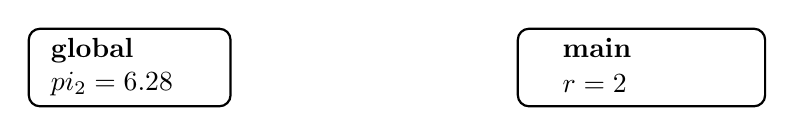
\begin{tikzpicture} [->, >= stealth']
	 	
	 	\node[state] (global)
		 	{

				\begin{tabular}{l}
					\textbf{global} \\
					\parbox{2cm}{
							$pi_2 = 6.28$}
				\end{tabular}
			};

		\node[state, text width=3cm, right of=global, node distance=6.5cm, anchor=center] (main)
			{	\begin{tabular}{l}
					\textbf{main} \\
					\parbox{2cm}{$r=2$}
					
				\end{tabular}
				
			};
%
%	 	
%	 	
%	 	
	 	\end{tikzpicture}
	 	
	 	\paragraph{Referenzen}
	 	
	 	\begin{itemize}
	 		\item sind neue (zusätzliche) Namen für vorhandene Speicherzellen
	 		
	 		\begin{lstlisting} [tabsize = 2]
		 		int x = 3;   // neue Variable x mit neuer Speicherzelle
		 		int & y = x; // Referenz: y ist neuer Name fuer x, beide haben dieselbe Speicherzelle
		 		
		 		y = 4; // Zuweisung an y, aber x aendert sich auch, d.h. x == 4
		 		x = 5; // jetzt y == 5
		 		
		 		int const & z = x; // read-only Referenz, d.h. z = 6 ist verboten
		 		x = 6;   // jetzt auch z == 6
	 		\end{lstlisting}
	 		\item Hauptanwendung:
	 		\begin{itemize}
	 			\item Umgebung, wo eine Funktion aufgerufen wird und die Umgebung der Implementation sind unabhängig, d.h. Variablen der einen Umgebung sind in der anderen nicht sichtbar
	 		\end{itemize}
	 		Beispiel: 
	 		\begin{lstlisting} [tabsize = 2]
		 		int foo (int x) {  // pass-by-value (Uebergabe des echten Werts)
			 		x += 3;
			 		return x;
		 		}
		 		
		 		int bar (int & x) {  // pass-by-reference (Uebergabe der Adresse der Speicherzelle)
			 		y += 3;
			 		return y;
		 		}
		 		
		 		void baz (int & z) {  // pass-by-reference
			 		z += 3;  // kein return Wert
		 		}
		 		
			 	int main() {
			 		int a = 2;
			 		std::cout << foo(a) << "\n";  // Ausgabe: 5
			 		std::cout << a << "\n";    // Ausgabe 2
			 		
			 		std::cout << bar(a) << "\n";  // Ausgabe: 5
			 		std::cout << a << "\n";   // Ausgabe: 5
			 		
			 		baz(a);
			 		std::cout << a << "\n";
		 		}
		 		
	 		\end{lstlisting}
	 		\item Funktionen die Werte nur über eine Referenz änder heißen Seiteneffekt der Funktion \\
	 		(Haupteffekt ist immer der return Wert) [in der funktionalen Programmierung sind Seiteneffekte verboten mit Ausnahme von Ein-/Ausgabe]

	 	\item Ziele
	 	\begin{enumerate}
	 		\item häufig möchte man Speicherzellen in beiden Umgebungen teilen $\Rightarrow$ verwende Referenzen
	 		\item häufig will man vermeiden, dass eine Variable kopiert wird (pass-by-value) \\
	 		$\Rightarrow$ durch \textit{pass-by-value} braucht man keine Kopie $\Rightarrow$ typisch $const \, \& \approxeq$ read-only, \underline{keine} Seiteneffekte
	 	\end{enumerate}
	 	
	 	\begin{lstlisting} [tabsize = 2]
	 		void print_string(std::string const & s) {
		 		std::cout << s;
	 		}
	 	\end{lstlisting}
	 \end{itemize}
	 
	 \section{Container-Datentypen}
	 dienen dazu, andere Datentypen aufzubewahren
	 \begin{itemize}
	 	\item Art der Elemente
	 	\begin{itemize}
		 	\item homogene Container: alle Elemente haben den gleichen Typ (typisch für $C++$)
		 	\item heterogene Container: Elemnte können verschiedene Typen haben (z.B. Python)
	 	\end{itemize}
	 	\item Art der Größe
	 	\begin{itemize}
	 		\item statische Container: feste Größe, zur Compilezeit bekannt
	 		\item dynamische Container: Größe zur Laufzeit veränderbar
	 	\end{itemize}
	 	\item Arrays sind die wichtigsten Container, weil effizient auf Hardware abgebildet und einfach zu benutzen
	 	\begin{itemize}
	 		\item klassisch: Arrays sind statisch, z.B. C-Arrays (hat $C++$ geerbt)
	 		\item modern: dynamische Arrays:
	 		\begin{itemize}
	 			\item Entdeckung einer effizienten Implementierung
	 			\item Kapselung durch Objekt-Orientierte-Programmierung (sonst zu kompliziert)
	 		\end{itemize}
	 	\end{itemize}
	 	\item ein dynamisches Array: $std::string$ ist Abbildung $int \rightarrowtail char \quad Index \rightarrow Zeichen$
	 	\item wir wollen das selbe Verhalten für \underline{beliebige} Elementtypen: $std::vector$
	 \end{itemize}
	 	
	 	\paragraph{Datentyp: $std::vector$}
	 	
	 	\begin{itemize}
	 	\begin{lstlisting} [tabsize = 2]
	 		#include <vector>
	 		
	 		std::vector <double> v(20, 0.0) ;  // initialisiert mit Groesse, Initialwert
	 		
	 		// analog: std::vector<int>, std::vector<std::string>
	 	\end{lstlisting}
	 	\item Abbildung: $int \rightarrowtail double$
	 	
	 	\item weitere Verallgemeinerung: Indextyp beliebig (man sagt dann "'Schlüssel-Typ§"' \\
	 	typische Fallen:
	 	\begin{itemize}
	 		\item Index ist nicht im Bereich $0 \leq Index < size$ ,z.B. Matrikelnummer
	 		\item Index ist String, z.B. Name eines Studenten
	 	\end{itemize}
	 	\item $std::map, \, std::unordered_map$ (Binärer Suchbaum) \\ \\
	 	 Beispiel:
	 	 \begin{lstlisting} [tabsize = 2]
	 	 	std::map <int, double> noten;  // noten[3 1 2 4 5  2 3 1 3] = 1.0
	 	 	std::map <string, double> noten;  // noten["krause] = 1.0
	 	 \end{lstlisting}
	 	 dabei: <Schlüsseltyp, Elementtyp>
	 \end{itemize}
	 
	 \begin{itemize}
	 	\item Erzeugen:
	 	\begin{lstlisting} [tabsize = 2]
	 		std::vector <double> v(20, 1.0);
	 		std::vector <double> v;   // leeres Array (erst ab C++ 11)
	 		
	 		std::vector <double> v = {1.0, -3.0, 2.2};  // "initializer list"
	 	\end{lstlisting}
	 	\item Größe:
	 	\begin{lstlisting} [tabsize = 2]
	 		v.size()
	 		v.empty()  (=v.size() ==0)
	 	\end{lstlisting}
	 	\item Größe ändern:
	 	\begin{lstlisting} [tabsize = 2]
	 		v.resize(neue_groesse, initialwert)
			 	1.: neue_gr < size()  // Elemente ab neue_gr geloescht, andere bleiben
			 	2.: neue_gr > size()  // neue Elemente mit Initialwert am Ende angehaengt
			 	
	 		v.push_back(neues_element)  // ein neues Element am Ende anhaengen
	 		
	 		v.insert(v.begin+index, neues_element); // neues Element an Position
								 		// index einfuegen folgende Werte werden 
								 		// um eine Position verschoben
				 	v.begin() ist Iterator
		 	
		 	v.pop_back()  // letztes Element loeschen (effizient)
		 	
		 	v.erase(v.begin()+index)  // Element aus Position loeschen, 
										 	// hintere Werte verschieben
		 	
		 	v.clear()  // alles loeschen
	 	\end{lstlisting}
	 	\item Zugriff:
	 	\begin{lstlisting} [tabsize = 2]
	 		v[k]  // Element bei Index k
	 		v.front()  // erstes Element
	 		v.back()  // letztes Element
	 		
	 		v.at(k)  // wie v[k], aber Fehlermeldung, wenn nicht 0<= k < size()
	 	\end{lstlisting}
	 	\item Funktionen für Container: benutzen in $C++$ Iteration, damit sie für verschiedenste Container funktionieren
	 	\item Iteration-Range: 
	 	\begin{lstlisting} [tabsize = 2]
	 		v.begin()
	 		v.end()  // hinter dem letzten Element
	 		
	 		im Header <algorithm>
	 	\end{lstlisting}
	 	\item alle Elemente kopieren:
	 	\begin{lstlisting} [tabsize = 2]
	 		std::vector <double> source = {1.0, 2.0, 3.0, 4.0, 5.0};
	 		std::vector <double> target(source.size(), 0.0);
	 		
	 		std::copy(source.begin(), source.end(), target.begin());
	 		std::copy(source.begin()+2, source.end(), target.begin());  
			 		// unbenutzte Initialwerte bleiben erhalten
	 	\end{lstlisting}
	 	\item Elemente sortieren:
	 	\begin{lstlisting} [tabsize = 2]
	 		std::sort(v.begin(), v.end());  // "in-place"
	 		std::random_shuffle(v.begin(), v.end())  // "in-place"
	 	\end{lstlisting}
	 \end{itemize}
	 
	 \paragraph{Warum ist $push\_back()$ effizient?}
	 
	 \begin{itemize}
	 	\item veraltete Lehrmeinung: Arrays sind nur effizient, weenn statisch (d.h. Größe zur Compilezeit, spätestens bei Initialisierung bekannt)
	 	\item modern: bei vielen Anwenduungen genügt, wenn Array (meist) nur am Ende vergrößert wird (z.B. $push\_back$) \\
	 	dies kann sehr effizient unterstützt werden $\Rightarrow$ dynamisches Array
	 	\item $std::vector$ verwaltet intern ein statisches Array der Größe "'$v.capacity() >= v.size()$"'
	 	\begin{itemize}
	 		\item wird das interne Array zu klein $\Rightarrow$ wird automatisch auf ein doppelt so großes umgeschaltet
	 		\item ist das interne Array zu groß, bleiben unbenutzte Speicherzellen als Reserve
	 	\end{itemize}
	 	\item Verhalten bei $push\_back()$
	 	\begin{itemize}
	 		\item noch Reserve vorhanden: lege neues Element in eine unbenutzte Speicherzelle $\Rightarrow$ billig \& chillig
	 		\item keine Reserve: 
	 		\begin{enumerate}
	 			\item alloziere neues statisches Array mit doppelter Kapazität
	 			\item kopiere die Daten aus allem ins neue Array
	 			\item gebe das alte Array frei
	 			\item gehe zu  \kreis{1}, jetzt wieder Reserve vorhanden \\ Umkopieren ist nicht teuer, da es nur selten nötig ist
	 		\end{enumerate}
	 		\item Beispiel:
	 		\begin{lstlisting}
	 			std::vector <int> v;
	 			for (int k = 0; k < 32; ++k) {
	 			v.push_back(k);
	 			}
	 		\end{lstlisting}
	 		\begin{tabular} {c|c|c|c|c|c}
		 		k & $cap\, vor \, p\_b()$ & $cap\, nach \, p\_b()$ & $size()$ & Reserve & Umkopierung \\
		 		\hline
		 		0 & 0 & 1 & 1 & 0 & 0 \\
		 		1 & 1 & 2 & 2 & 0 & 1 \\
		 		2 & 2 & 4 & 3 & 1 & 2 \\
		 		3 & 4 & 4 & 4 & 0 & 0 \\
		 		4 & 4 & 8 & 5 & 3 & 4 \\
		 		5 $\dots$ 7 & 8 & 8 & 8 & 0 & 0 \\
		 		8 & 8 & 16 & 9 & 7 & 8 \\
		 		9 $\dots$15 & 16 & 16 & 16 & 0 & 0 \\
		 		16 & 16 & 32 & 17 & 15 & 16 \\
	 		\end{tabular} \\ \\
	 				 		$\cdots$
	 	\end{itemize}
	 	
	 	\item Kosten:
	 	\begin{itemize}
	 		\item 32 Elemente einfügen $=$ 32 Kopien extern $\Rightarrow$ intern
	 		\item aus altem Array ins neue kopieren $=$ 31 Kopien intern $\Rightarrow$ intern \\
	 		$\Rightarrow$ im Durchschnitt sind pro Einführung 2 Kopien nötig \\
	 		$\Rightarrow$ dynamisches Array ist doppelt so teuer, wie das statische \\
	 		$\Rightarrow$ immer noch sehr effizient
	 	\end{itemize}
	 	\item relevante Funktionen von $std::vector$
	 	\begin{itemize}
	 		\item $v.size()$: aktuelle Zahl der Elemente
	 		\item $v.capacity()-v.size()$: Reserve ($\geq 0$)
		 	\item $v.resize(new\_size)$: ändert immer $v.size()$, aber $v.capacity()$ nur wenn $< new\_size$
		 	\item $v.reserve(new\_capacity)$: ändert $v.size()$ nicht, aber $v.capacity()$ falls $new\_capacity \geq size$
		 	\item $v.shrink\_to\_fit()$: $v.reserve(v.size())$ (Reserve ist danach 0), wenn Endgröße erreicht
	 	\end{itemize}
	 	\item wenn Reserve $> size$: $capacity$ kann auch halbiert werden
	 \end{itemize}
	 
	 \paragraph{wichtige Container der $C++$ Standardbiblithek}
	 
	 \begin{itemize}
	 	\item dynamisches Arrays: $std::string, std::vector$
	 	\item assoziative Arrays: $std::map, std::unordered\_map$
	 	\item Mengen: $std::set, std::unordered\_set$ (jedes Element ist höchstens einmal enthalten)
	 	\item Stapel: $std::stack$ (Funktion: "'last-in-first-out"') z.B. gestapelte Bierkästen.
	 	\item Warteschlange: $std::queue$ (Funktion: "'first-in-first-out"')
	 	\item Kartendeck: $std::deque$ gleichzeitig Stapel und Warteschlange
	 	\item Stapel mit Priorität: $std::priority\_queue$ (Priorität vom Nutzer definiert)
	 \end{itemize}
	 	
	 \section{Iteratoren}
	\begin{itemize}
		\item für Arrays lautet kanonische Schleife:
		\begin{lstlisting} [tabsize = 2]
			for (int k = 0; k != v.size(); ++k) {
				int current = v[k];  // aktuelles Element lesen
				v[k] = new_value;  // aktuelles Element schreiben
			}
		\end{lstlisting}
		\item wir wollen eine so einfache Schleife für beliebige Container
		\begin{itemize}
			\item der Index-Zugriff $v[k]$ ist bei den meisten Containern nicht effizient
			\item Iteratoren sind immer effizient $\Rightarrow$ es gibt sie in allen modernen Programmiersprachen, aber die Details sind sehr unterschiedlich
			\item Analogie: Zeiger einer Uhr, Cursor in Textverarbeitung \\
			$\Rightarrow$ ein Iterator zeigt immer auf ein Element des Containers oder auf Spezialwert "'ungültiges Element"'
			\item in $C++$ unterstützt jeder Iterator 5 Grundoperationen
			\begin{enumerate}
				\item Iterator auf erstes Element erzeugen:
				\begin{lstlisting} [tabsize = 2]
					auto iter = v.begin();  // auto ist Universaltyp, wird 
													// vom Compiler automatisch
													//  mit richtigen Typen ersetzt
				\end{lstlisting}
				\item Iterator auf "'ungültiges Element"' erzeugen:
				\begin{lstlisting} [tabsize = 2]
					auto end = v.end()  // typischerweise v[v.size()]
				\end{lstlisting}
				\item Vergleich:
				\begin{lstlisting} [tabsize = 2]
					iter1 == iter2;
					iter != end;  (= !(iter == end))  // iter zeigt nicht auf
																  // ungueltiges Element
				\end{lstlisting}
				\item zum nächsten weitergehen: $++iter$, Ergebnis ist $v.end()$, wenn man vorher beim letzten Element war
				\item auf Daten des aktuellen Elements zugreifen: $*iter$ ("'Dereferenzierung"')
			\end{enumerate}
		\end{itemize}
		\item $\Rightarrow$ kanonische Schleife:
		\begin{lstlisting} [tabsize = 2]
			for (auto iter = v.begin(); iter != v.end(); ++iter) {
				int current = *iter;  // lesender Zugriff;
				*iter = new_value;  // schreibender Zugriff
				
				// Abkuerzung in C++: rang-based for-loop
				for (int & element : v) {
					int current = element;  // lesen
					element = new_value;  // schreiben
				}
			}
		\end{lstlisting}
		\item wenn die zugrunde liegenden Speicherzellen geändert werden, also die Containergröße sich ändert, werden die Iteratoren ungültig
		\item Iteratoren mit den 5 Grundoperationen heißen "'forward iterators"' (wegen $++iter$)
		\item "'bidirectional iterators"' unterstützen auch $--iter$ (alle Iteratoren aus Standardbibliothek)
		\item "'random access iterators"' können beliebige Sprünge machen ($iter+=5$) \\
		unterstützt von $std::string$ und $std::vector$
		\item Besonderheit für assoziative Arrays ($std::map$):
		\begin{itemize}
			\item Schlüssel und Werte können beliebig gewählt werden \\
			$\Rightarrow$ das aktuelle Element ist immer ein Schlüssel/Wert-Paar \\
			$(*iter).first \Rightarrow$ Schlüssel \\
			$(*iter).second \Rightarrow$ Wert
			\begin{lstlisting} [tabsize = 2]
				v[(*iter).first] == (*iter).second;
			\end{lstlisting}
		\end{itemize}
		\item Bei $std::map$ liefern die Iteratoren die Elemente in aufsteigender Reihenfolge der Schlüssel (Unterschied zu $std::unordered\_map$)
	\end{itemize}
	
	
	
	
\end{document}